\documentclass{beamer}
\begin{document}
\title{Python Chapter 1}
\author{Ezequiel Torres}
\date{\today}
\frame{\titlepage}
\frame{\frametitle{Table of contents}\tableofcontents}

\section{Before getting started}
\frame{\frametitle{Before getting started}
    We will be going over the basics of python and interviewing in python in this course.
    Here are some great resources to get started.
    \begin{itemize}
        \item<1-> http://programarcadegames.com
            \begin{itemize}
                \item<2-> Fun way to learn python at your own pace while making arcade games!
            \end{itemize}
        \item<3-> https://www.crackingthecodinginterview.com/
            \begin{itemize}
                \item<4-> 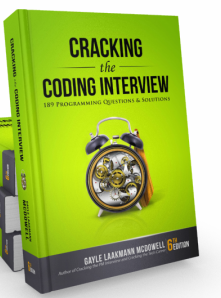
\includegraphics{CTCI.png}
            \end{itemize}
    \end{itemize}
}
\frame{\frametitle{Before getting started}
    \begin{itemize}
        \item<1-> https://www.amazon.com/Grokking-Algorithms-illustrated-programmers-curious/dp/1617292230
            \begin{itemize} 
                \item<2-> 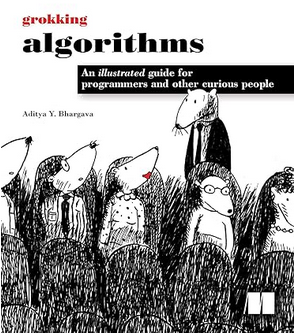
\includegraphics{ga.png}
            \end{itemize}
        \item<3-> https://github.com/zeaktorres/WSU-Python-Workshop-2024/
            \begin{itemize}
                \item<4-> Where the notes will be stored 
            \end{itemize}
    \end{itemize}
}
\section{Variables}
\frame{\frametitle{Variables} 
    Here we will go into some basic examples of variables in python.
    First variables should be lowercase
    \begin{enumerate}
        \item<1-> x = 5
        \item<1-> y = 10
        \item<1-> print(x + y)
    \end{enumerate}
    15
}
\subsection{Variables and Concatenation}
\frame{\frametitle{Variables and Concatenation} 
    "In formal language theory and computer programming, string concatenation is the operation of joining character strings end-to-end" - Wikipedia
    IE: print("Hello" + "World")
}
\subsection{Variables Exercise}
\frame{\frametitle{Variables Exercise}
    Write a python program which prints a users mpg. You can take in input in python like the following:
    miles_driven = input('Enter the number of gallons')
    Note: These exercises are purposly vague as are interview questions to get you to ask important questions
    Note: Sometimes interviewers will give you hints if you are struggling but some interviewers will take taking a hint as a negative
}



\end{document}
